%******************************************************************************%
%                                                                              %
%                  JavaScript.en.tex for LaTeX                                 %
%                  Created on : Tue Mar 10 13:27:28 2015                       %
%                  Made by : Don Stolz <dstolz@student.42.us.org>              %
%                                                                              %
%******************************************************************************%

\documentclass{42-en}


%******************************************************************************%
%                                                                              %
%                                    Header                                    %
%                                                                              %
%******************************************************************************%
\begin{document}
\title{JavaScript}
\member{Donald Stolz}{dstolz@student.42.us.org}
\summary {
 Setup a Heroku account and host your first remote server. 
}
\maketitle

\tableofcontents

%******************************************************************************%
%                                                                              %
%                                 Introduction                                 %
%                                                                              %
%******************************************************************************%
\chapter{Introduction}

So far we have been running our server from our local machine. We have had to manually start and stop our server when we want to access our API. Now we our going to host our server in the cloud using Heroku. That way Heroku will keep our server running and users can access the API whenever.

%******************************************************************************%
%                                                                              %
%                                Pre-req: Homebrew                             %
%                                                                              %
%******************************************************************************%
\chapter{Pre-req: Homebrew & Heroku CLI}

First we need to install Homebrew, so that we can later install the Heroku CLI\\

Copy and paste the following into your terminal.
\begin{42shell}
	mkdir $HOME/.brew && curl -fsSL https://github.com/Homebrew/brew/tarball/master | tar xz --strip 1 -C $HOME/.brew
	mkdir -p /tmp/.$(whoami)-brew-locks
	mkdir -p $HOME/.brew/var/homebrew
	ln -s /tmp/.$(whoami)-brew-locks $HOME/.brew/var/homebrew/locks
	export PATH="$HOME/.brew/bin:$PATH"
	brew update && brew upgrade
\end{42shell}

Afterwards make sure you add the following lines to your `.zshrc`.\\
You can access this file by using `vim .zshrc`
\begin{42shell}
	mkdir -p /tmp/.$(whoami)-brew-locks
	export PATH="$HOME/.brew/bin:$PATH"
\end{42shell}

Once we have Homebrew installed we can install the Heroku. Simply run:
\begin{42shell}
$ brew tap heroku/brew && brew install heroku
\end{42shell}


\newpage
%******************************************************************************%
%                                                                              %
%                                  Instructions                                %
%                                                                              %
%******************************************************************************%
\chapter{Instructions}

First head to \href{https://www.heroku.com/}{https://www.heroku.com/} and click signup

\begin{figure}[H]
    \begin{center}
        
\includegraphics[width=14cm]{WEB/heroku_0.png}
    \end{center}
\end{figure}

Fill out the simple form to create an account
\begin{figure}[H]
    \begin{center}
        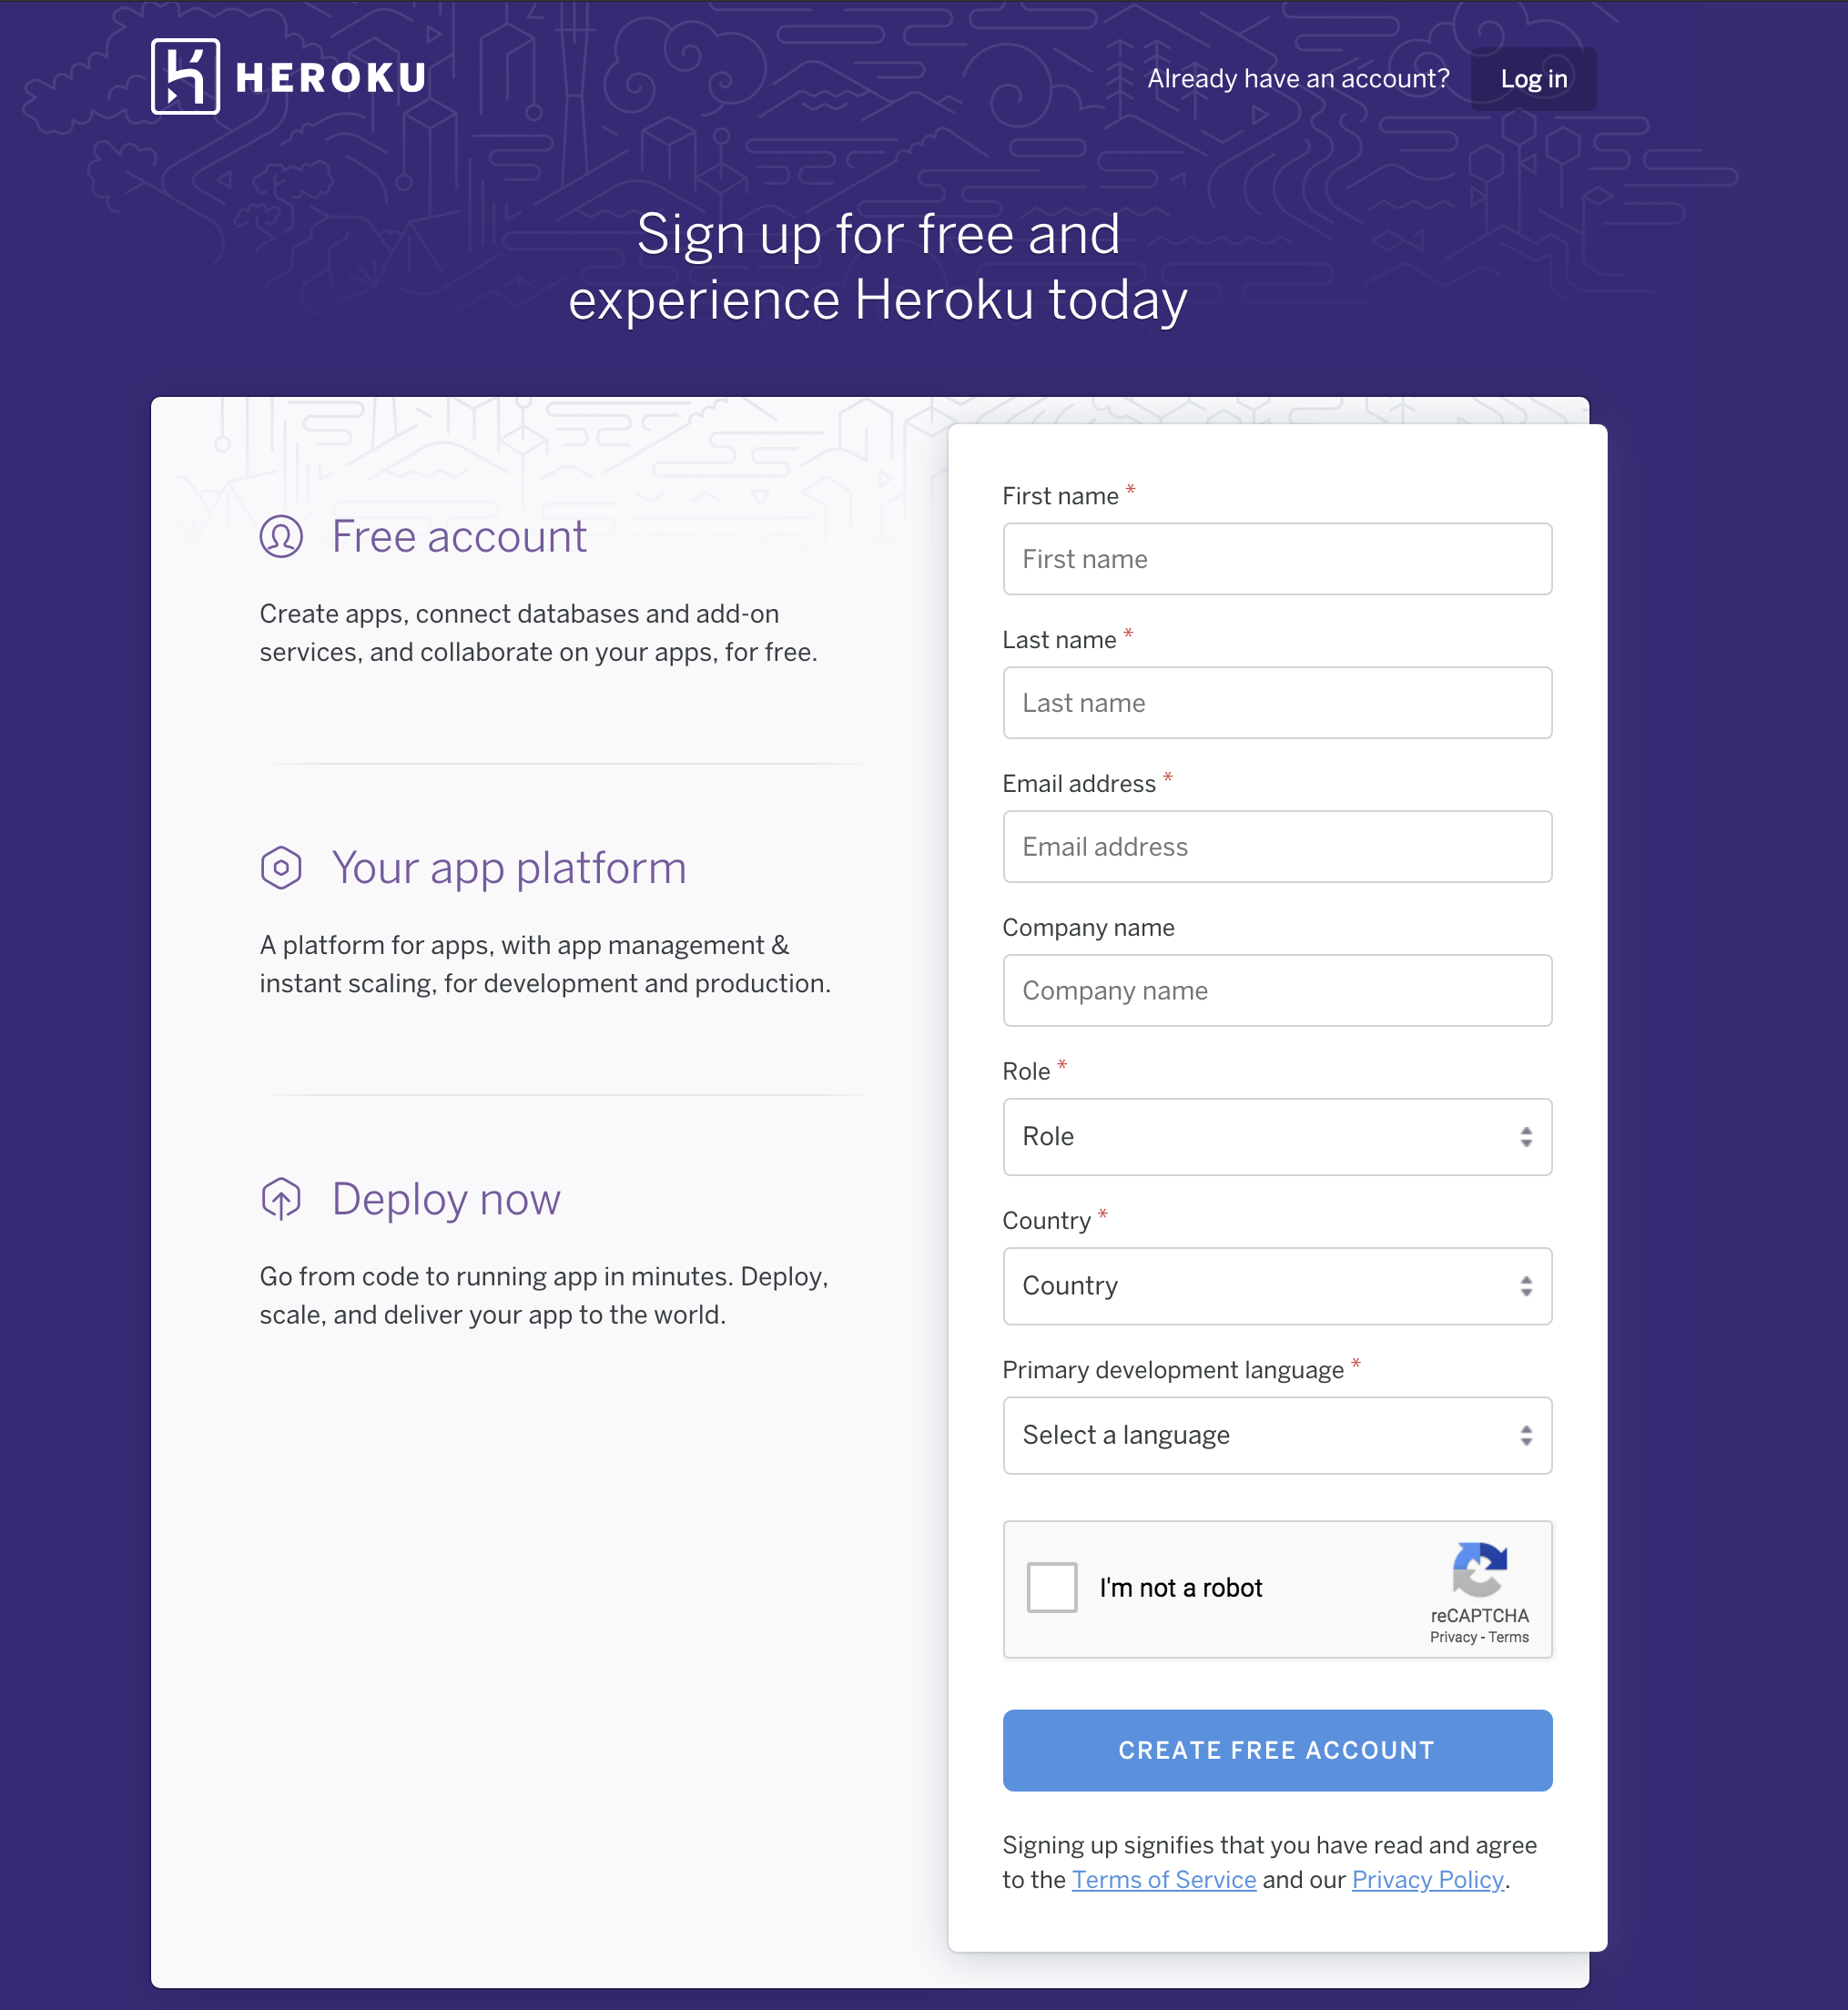
\includegraphics[width=14cm]{WEB/heroku_1.png}
    \end{center}
\end{figure}

\newpage

Next head to `create new app`
\begin{figure}[H]
    \begin{center}
        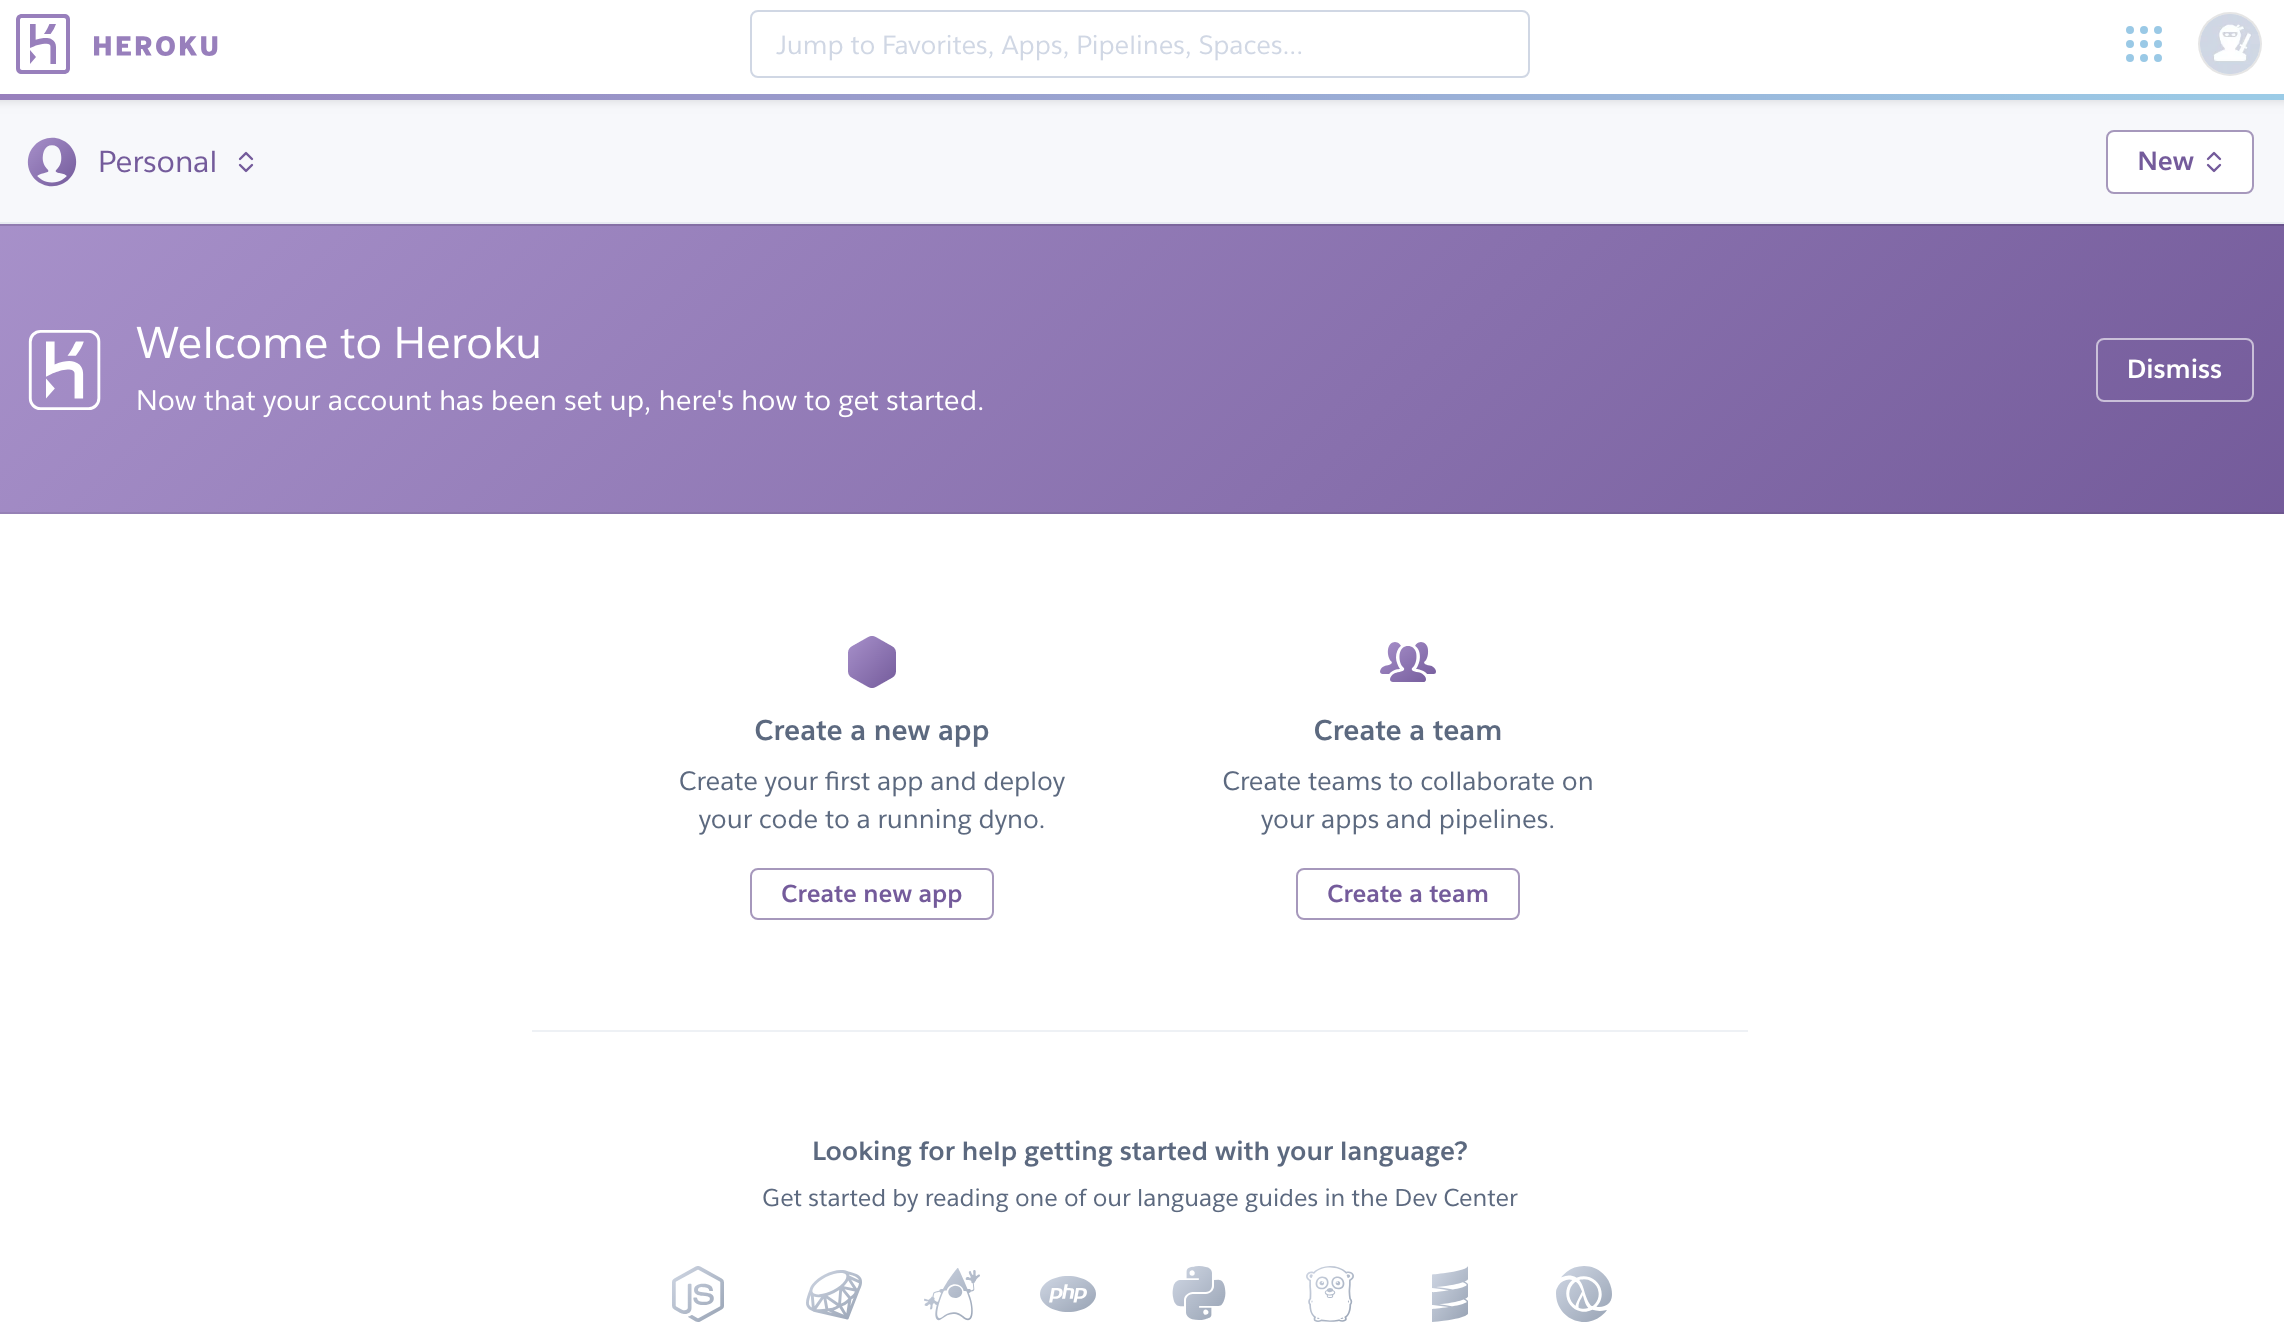
\includegraphics[width=12cm]{WEB/heroku_2.png}
    \end{center}
\end{figure}

Simply give your app a name
\begin{figure}[H]
    \begin{center}
        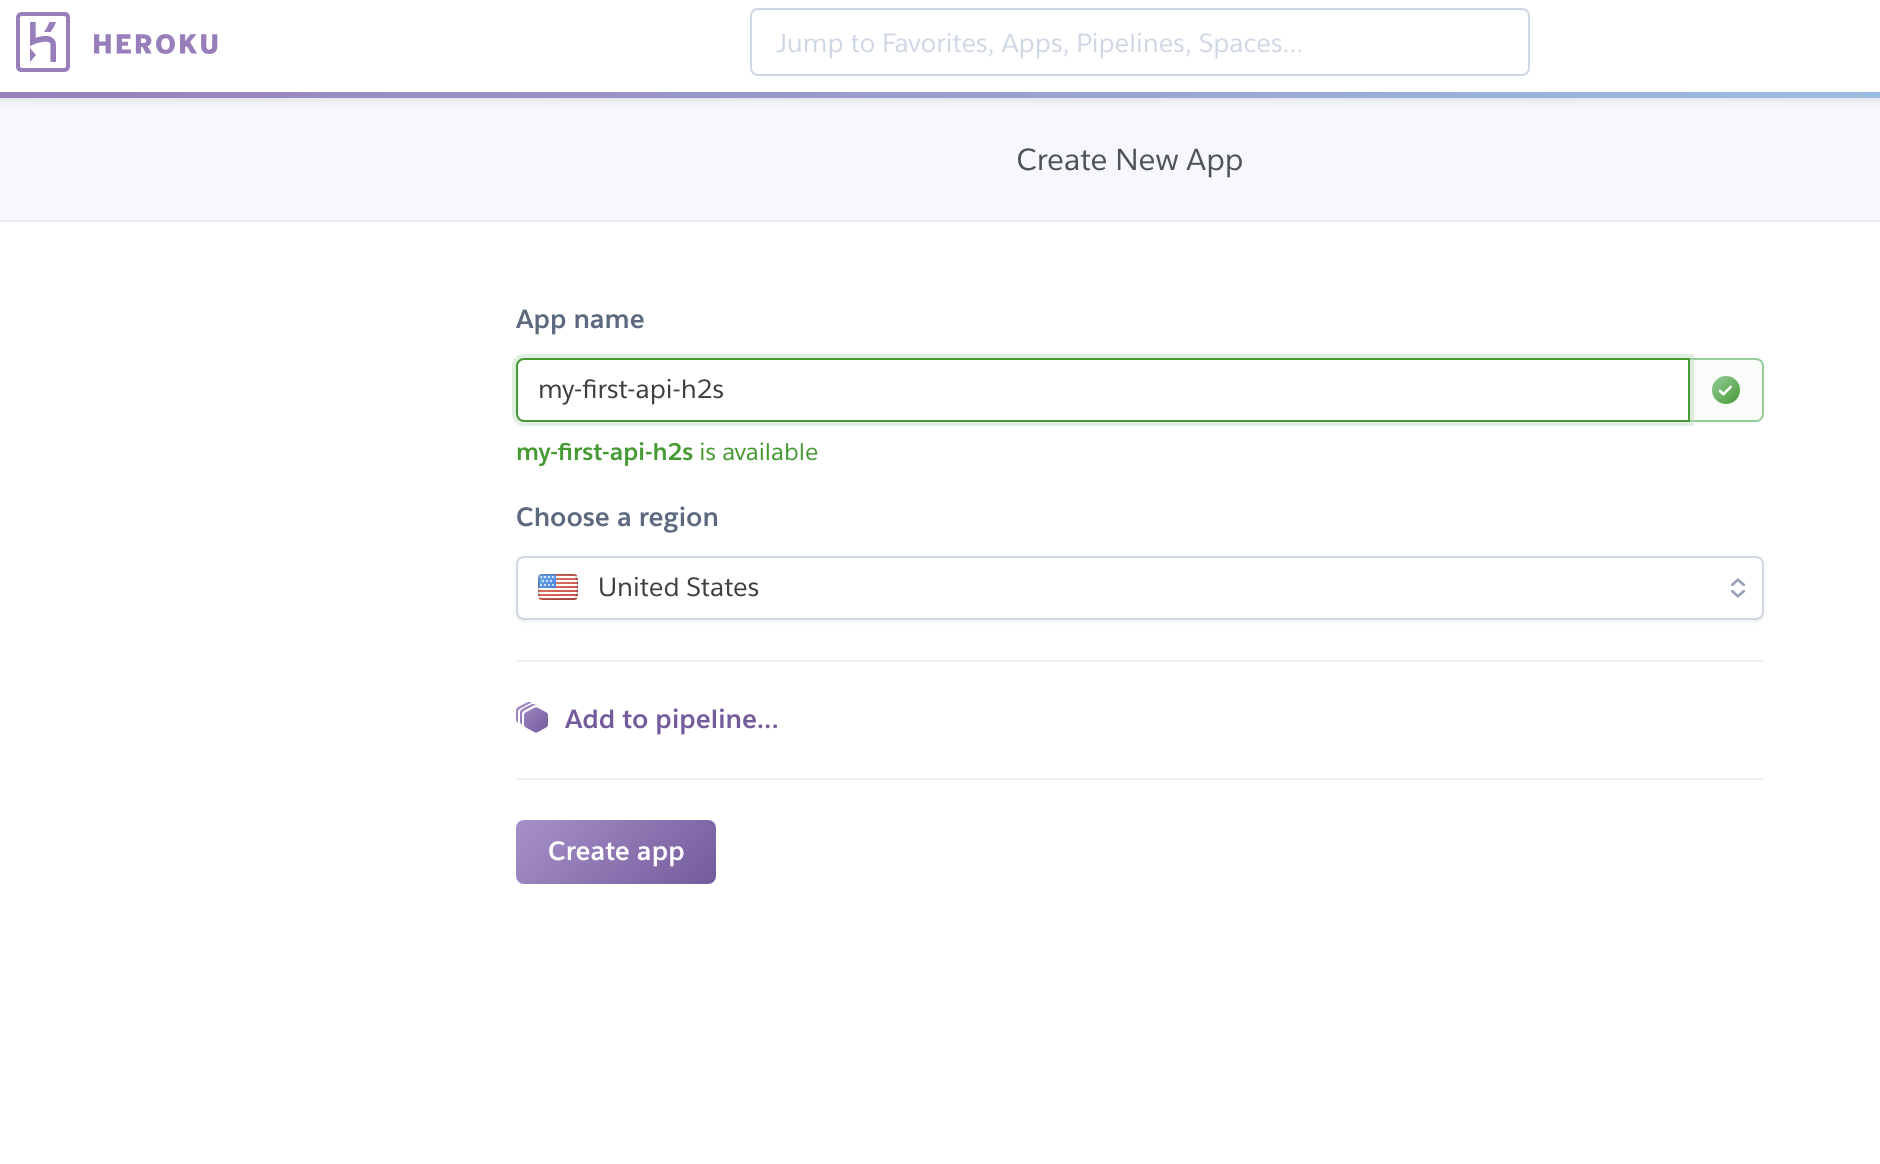
\includegraphics[width=14cm]{WEB/heroku_3.png}
    \end{center}
\end{figure}

\newpage

Once you get to this page you will need to login to the Heroku cli. Then copy your command to add heroku to an `Existing Git repository`. Finally follow the `Deploy your application` instructions.
\begin{figure}[H]
    \begin{center}
        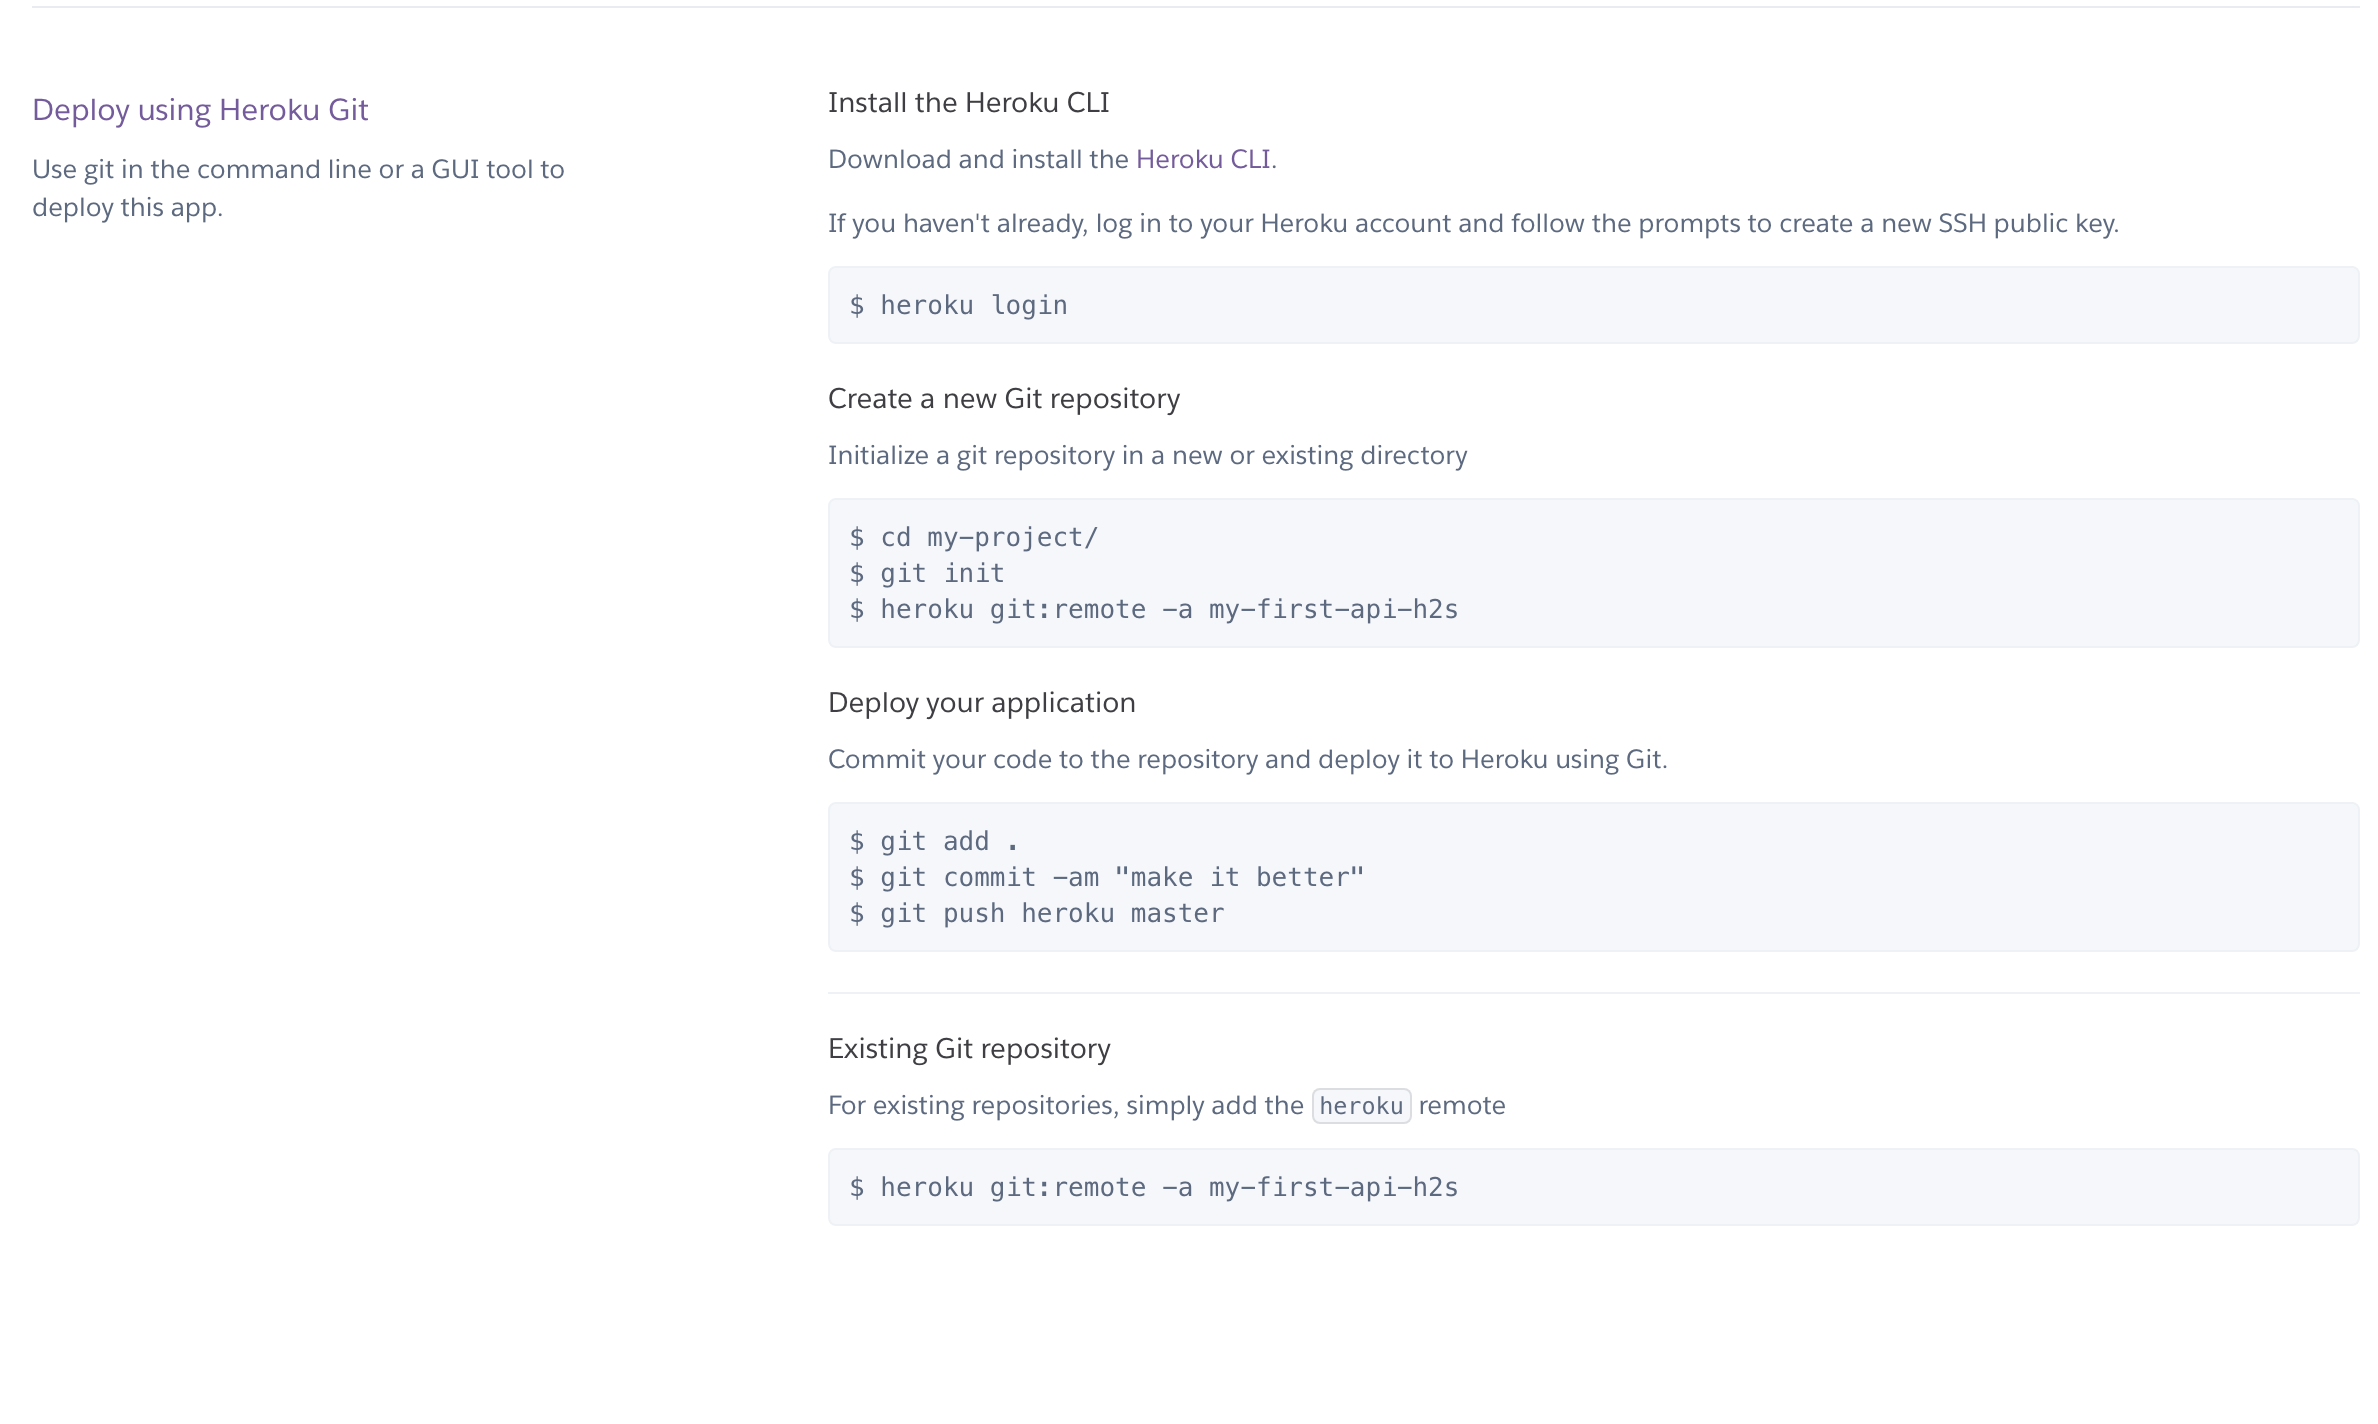
\includegraphics[width=14cm]{WEB/heroku_4.png}
    \end{center}
\end{figure}

%******************************************************************************%
\end{document}